\documentclass[12pt, a4paper, twoside]{article}

%% Preamble
\usepackage{pdfpages}           % Para incluir PDFs
\usepackage{graphicx}           % Para gráficos
\usepackage{subfiles}           % Para manejar subarchivos
\usepackage{hyperref}           % Para enlaces
\usepackage{listings}           % Para código fuente (ajusta lenguaje)
\usepackage{verbatim}
\usepackage[backend=bibtex,style=numeric]{biblatex} % Para citas numéricas
\addbibresource{references.bib} % Cargar archivo .bib
\usepackage{url}


\usepackage{geometry}           % Para ajustar márgenes

% Ajustes de márgenes
\geometry{
	left=3cm,       % Margen izquierdo
	right=3cm,      % Margen derecho
	top=2.5cm,      % Margen superior
	bottom=2.5cm,   % Margen inferior
	headheight=15pt, % Altura del encabezado
	twoside          % Para documentos a dos caras
}


\graphicspath{{images/}{../images/}} % Ruta para imágenes

\begin{document}
	
	%% Cover
	
\includepdf[noautoscale=true, width=\paperwidth]{cover.pdf}
	
	%% Title
	\clearpage
	\setcounter{page}{1}
	
\includepdf[noautoscale=true, width=\paperwidth]{title.pdf}
	
	%%%%%%%%%%%%%%%%%%%%%%%%%%%%%%%%%%%%%%%%%%%%%%%%%%%%%%%%%%%%%%%%%%%%%%%%%%%
	
	% Índice automático
	\tableofcontents
	\newpage
	
	% Sections
	
		% Sections
	\section{Introducción}
	
	El diseño y desarrollo de \textbf{almacenes de datos} es crucial para el análisis clínico, mejorando la toma de decisiones médicas y la calidad de atención a los pacientes. Para este proyecto, se utilizará una visión parcial de un almacén de datos basado en la \textit{Base de Datos de Investigación Colaborativa eICU}, la cual contiene una vasta cantidad de información sobre los ingresos en \textbf{Unidades de Cuidados Intensivos (UCI)} en diversos hospitales de los Estados Unidos.\cite{futuro}
	
	El enfoque de este trabajo está dirigido específicamente a los \textbf{pacientes con problemas respiratorios}. Estos casos son de especial relevancia en entornos de cuidados críticos, ya que las afecciones respiratorias representan una de las principales causas de ingreso en las UCI. Por lo cual un almacén de datos centrada en estas patologías sigue representando una gran fuente de información y con mucho interés para hacer un análisis de datos. \cite{pekar2021epidemiology, vincent2006epidemiology}.
	
	En este trabajo, el \textbf{hecho principal} está constituido por los ingresos en la UCI, complementado por un conjunto de dimensiones que permiten analizar diversas variables. La selección de las tablas y atributos más relevantes de la base de datos eICU será el mayor reto para construir un \textbf{almacén de datos eficiente y de interés analítico}, que no solo facilite la consulta de información clave,
	a su vez soporte y facilité tanto la investigación clínica como la optimización de los protocolos de tratamiento.
	
	\section{Objetivos}
	
	El objetivo de este trabajo es desarrollar un \textbf{diseño conceptual y lógico} de un almacén de datos centrado en los pacientes ingresados en la \textbf{UCI} con afecciones respiratorias, seleccionando las partes más relevantes de la base de datos para el análisis de estas patologías.
	
	Se procederá a la restauración de dicha base de datos en \textit{SQL Server}, para realizar una selección de las tablas más relevantes que contribuyan a la construcción del almacén de datos centrado en estos pacientes. En cada una de las tablas seleccionadas, se identificarán los atributos más significativos para el análisis clínico y el seguimiento de los pacientes con problemas respiratorios. 
	
	Una vez completada la selección de dimensiones y tablas de hechos, se diseñará el modelo conceptual utilizando la herramienta \textit{draw.io}, y posteriormente se desarrollará el modelo lógico mediante un diagrama de base de datos en el entorno de \textit{SQL Server}. 
	
	\section{Descripción de los datos utilizados (eICU)}
	
	 La base de datos \textit{eICU-CRD}, desarrollada por el Philips eICU Research Institute (eRI), contiene datos desidentificados de pacientes ingresados en Unidades de Cuidados Intensivos (UCI). Esta base de datos, que forma parte del programa de telesalud en cuidados críticos de Philips, documenta detalles sobre diagnósticos, tratamientos, pruebas y resultados.
	
	La \textit{eICU-CRD} recopila una amplia cantidad de datos clínicos con fines de investigación, permitiendo estudiar los resultados de los pacientes, identificar tendencias clínicas y evaluar protocolos de mejores prácticas utilizados en distintos centros de atención médica. Esta base de datos tiene como fin facilitar la investigación para mejorar la calidad de la atención en UCI.
	
	La \textit{eICU-CRD} contiene un total de 31 tablas, que agrupan 391 columnas de datos y un total de 457,325,320 filas. Esta vasta cantidad de información abarca diversos aspectos clínicos, como datos demográficos de los pacientes, información clínica obtenida durante el ingreso, pruebas y diagnósticos realizados, tratamientos y terapias administradas, así como la evolución y resultados durante la estancia en la UCI. Dada la magnitud de los datos. En este trabajo, se ha optado por simplificar el almacén, enfocándose en aquellos datos más relevantes para el análisis de pacientes ingresados en la UCI con problemas respiratorios. A continuación, se presentan las 9 tablas seleccionadas del almacén original:
	
	\begin{itemize}
		\item \texttt{ApacheApsVar:} Contiene diversas métricas utilizadas para evaluar la gravedad de la enfermedad de los pacientes al ingreso en la UCI como parte del sistema APACHE.
		
		\item \texttt{Admissiondx:} Contiene el diagnóstico principal por el cual el paciente fue admitido en la UCI, de acuerdo con los criterios de puntuación APACHE.
		
		\item \texttt{Allergy:} Contiene información sobre las alergias del paciente.
		
		\item \texttt{Diagnosis}: Contiene los diagnósticos documentados para cada paciente. Permite identificar las enfermedades documentadas durante la estancia en UCI, así como el momento en que se registraron.
		
		\item \texttt{Hospital:} contiene información sobre los hospitales participantes en el programa y sus pacientes vinculados.
		
		\item \texttt{Medication:} Contiene las órdenes activas de medicamentos para los pacientes.
		
		\item \texttt{Patient:} Contiene los datos demográficos del paciente, así como los detalles de su admisión y alta del hospital y la UCI.
				
		
		\item \texttt{RespiratoryCare:} Contiene información sobre el cuidado respiratorio.

		\item \texttt{RespiratoryCharting:} Contiene datos sobre la configuración respiratoria, como el tipo de gráfico y valores respiratorios.


	\end{itemize}

	
	
	Además de reducir el número de tablas también se encontró oportuno reducir el número de atributos de las mismas, al contener información poco esencial o que no se ve utilidad para las siguientes fases del trabajo. (Vea la figura \ref{fig:conceptual} para detallar las tablas y sus atributos de manera global)
	
	
	
	\section{Diseño conceptual}
	
	El diseño conceptual define las entidades, relaciones y requisitos de información de manera abstracta, sin detalles técnicos. Se enfoca en representar las necesidades y cómo organizar los datos para soportar la toma de decisiones.
	
	Recordando que se modela un almacén
	que trata sobre una población de \textbf{pacientes con problemas respiratorios} las tablas elegidas son las siguientes:
	
	%En este apartado se explicará la relevancia de cada tabla y atributos.
	
	
	\begin{figure}[h!]
		\begin{center}  % Usamos el entorno 'center'
			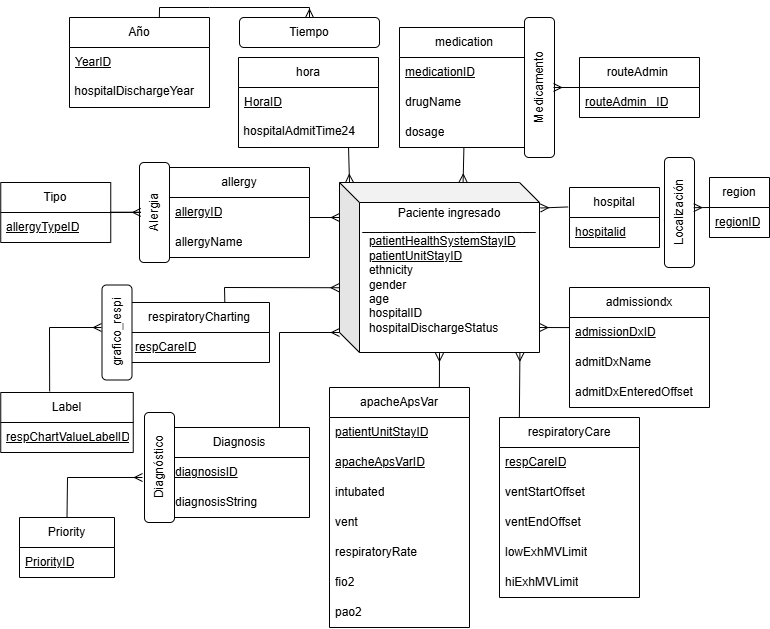
\includegraphics[width=1\textwidth]{image/diseno_conceptual.png}
			\caption{Diseño conceptual}
			\label{fig:conceptual}
		\end{center}
	\end{figure}
	
	%\vspace{-20pt} % Ajusta este valor para reducir el espacio
	
	
	\subsection{Tablas}
	
	\subsubsection{PacienteIngresado}
	
	
	
	\begin{itemize}
		\item \textbf{Relevancia}: La tabla \texttt{pacienteIngresado} es el hecho que almacena información demográfica de los pacientes y detalles relacionados con sus ingresos y egresos del hospital y la UCI. Es fundamental para el análisis de la estancia en la UCI y la hospitalización, proporcionando una visión global de la evolución clínica y de los tiempos de atención.
		
		\item \textbf{Selección de atributos}:
		\begin{itemize}
			\item \texttt{patientUnitStayID}: Clave primaria que identifica de manera única la estancia del paciente en la UCI. Relaciona con el registro de \texttt{patient} mediante este identificador.
			\item \texttt{patientHealthSystemStayID}: Identificador del ingreso hospitalario, vincula las estancias hospitalarias de un paciente durante un mismo periodo.
			\item \texttt{ethnicity}: Etnia del paciente, una variable importante para el análisis demográfico y la disparidad en la atención.
			\item \texttt{gender}: Género del paciente, relevante para estudios epidemiológicos y de salud pública.
			\item \texttt{age}: Edad del paciente, crucial para la estratificación del riesgo y el análisis de comorbilidades.
			\item \texttt{hospitalID}: Identificador único del hospital, esencial para la segmentación por centro de atención.
			\item \texttt{hospitalDischargeStatus}: Estado del paciente al momento del alta hospitalaria, indicando si está vivo, fallecido, o en otro estado.
			\item \texttt{hospitalAdmitTime24}: Hora exacta del ingreso al hospital, importante para el análisis temporal de la atención.
			\item \texttt{hospitalDischargeYear}: Año de alta hospitalaria, relevante para la evaluación de tendencias a lo largo del tiempo.
			\item \texttt{UniquePID}: Identificador único del paciente, utilizado para distinguir a los pacientes en el sistema.
		\end{itemize}
		
	\end{itemize}
	
	Algunos atributos no se han incluido debido a la duplicación o irrelevancia en el contexto del hecho pacienteIngresado. Por ejemplo, \texttt{hospitalAdmitTime24} y \texttt{hospitalDischargeYear}  ya cubren la información temporal necesaria, por lo que atributos como \texttt{unitAdmitTime24}  y \texttt{unitDischargeTime24} no son necesarios en este nivel, ya que hacen referencia a eventos más específicos de la UCI, no del ingreso hospitalario. Igualmente, \texttt{wardID} y \texttt{unitType} se han excluido porque son detalles más relevantes para el contexto de la unidad de UCI, no para el hecho principal del paciente ingresado.  \cite{eICU2024}
	
	
	\subsubsection{Diagnosis} 
	
	\begin{itemize}
		\item \textbf{Relevancia}: La tabla \texttt{Diagnosis} es clave para analizar diagnósticos de enfermedades respiratorias en pacientes, permitiendo filtrar y clasificar las condiciones por severidad.
		
		\item \textbf{Selección de atributos}:
		\begin{itemize}
			\item \texttt{patientUnitStayID}: Relaciona el diagnóstico con un paciente específico en la UCI.
			\item \texttt{diagnosisID}: Clave primaria para diferenciar cada diagnóstico.
			\item \texttt{diagnosisString}: Descripción completa del diagnóstico para consultas específicas.
			\item \texttt{diagnosisPriority}: Indica la prioridad del diagnóstico (Primario, Mayor, Otro).
		\end{itemize}
	\end{itemize}
	
	No se han incluido atributos como \texttt{diagnosisOffset} e \texttt{ICD9Code} debido a que este proyecto se centra más en la naturaleza y prioridad del diagnóstico que en el tiempo específico de entrada o el código ICD-9. \cite{eICU2024}
	
	\subsubsection{respiratoryCharting}
	
	\begin{itemize}
		\item \textbf{Relevancia}: La tabla \texttt{RespiratoryCharting} es fundamental para el monitoreo de los valores respiratorios de los pacientes en UCI, especialmente en aquellos con enfermedades respiratorias graves.
		
		\item \textbf{Selección de atributos}:
		\begin{itemize}
			\item \texttt{patientUnitStayID}: Asocia los datos respiratorios con un paciente específico.
			\item \texttt{respCareID}: Identificador único del registro respiratorio.
			\item \texttt{respChartValueLabel}: Describe el tipo de valor respiratorio (ej. HR, I:E Ratio), útil para categorizar los datos.
		\end{itemize}
		
	\end{itemize}
	
	Se decidió que datos como \texttt{respChartOffset} y \texttt{respChartValue} añadían detalles muy específicos, estos se descartaron para enfocar la relevancia clínica general sobre estos detalles puntuales, ya que el objetivo es estudiar tendencias en vez del seguimiento minuto a minuto.\cite{eICU2024}
	
	\subsubsection{respiratoryCare}
	
	\begin{itemize}
		\item \textbf{Relevancia}: La tabla \texttt{RespiratoryCare} es clave para el análisis de los cuidados respiratorios proporcionados a los pacientes en la UCI, ya que permite evaluar las intervenciones de ventilación mecánica y otras terapias respiratorias.
		
		\item \textbf{Selección de atributos}:
		\begin{itemize}
			\item \texttt{patientUnitStayID}: Asocia el cuidado respiratorio a un paciente específico.
			\item \texttt{respCareID}: Identificador único para cada intervención de cuidado respiratorio.
			\item \texttt{ventStartOffset}: Refleja el inicio de la ventilación, crucial para analizar la relación entre el inicio de la intervención y la evolución del paciente.
			\item \texttt{ventEndOffset}: Indica el final de la ventilación, permitiendo estudiar la duración de las intervenciones respiratorias.
			\item \texttt{lowExhMVLimit}: Establece el límite inferior del volumen minuto expiratorio, importante para evaluar la efectividad de la ventilación.
			\item \texttt{hiExhMVLimit}: Define el límite superior del volumen minuto expiratorio, igualmente relevante para evaluar la capacidad de los sistemas respiratorios.
		\end{itemize}
		
	\end{itemize}
	
	Se han excluido atributos como \texttt{airwayType} y \texttt{cuffPressure} porque el estudio se centra en parámetros que permiten observar el impacto de la ventilación mecánica en la evolución de los pacientes y no tanto en los detalles técnicos de cada intervención.\cite{eICU2024}
	
	\subsubsection{apacheApsVar}
	
	\begin{itemize}
		\item \textbf{Relevancia}: La tabla \texttt{apacheApsVar} es esencial para el cálculo del \texttt{Acute Physiology Score} (APS) III, un sistema ampliamente utilizado para evaluar la gravedad de la enfermedad de los pacientes al ingreso en la UCI. Esta puntuación es parte del sistema \texttt{APACHE} para predecir los resultados de los pacientes críticos.
		
		\item \textbf{Selección de atributos}:
		\begin{itemize}
			\item \texttt{patientUnitStayID}: Relaciona a cada entrada de paciente en la UCI con su respectivo registro en la tabla de pacientes.
			\item \texttt{apacheApsVarID}: Clave primaria que identifica de manera única cada conjunto de variables de \texttt{APACHE APS}.
			\item \texttt{intubated}: Indica si el paciente fue intubado al momento de obtener el peor valor de gasometría (ABG), crucial para evaluar la necesidad de intervención respiratoria.
			\item \texttt{vent}: Indica si el paciente fue ventilado al momento de registrar la peor frecuencia respiratoria, reflejando la gravedad de la insuficiencia respiratoria.
			\item \texttt{respiratoryRate}: Refleja la frecuencia respiratoria más baja durante el período de \texttt{APACHE}, utilizada para medir la función respiratoria del paciente.
			\item \texttt{fio2}: Mide la fracción inspirada de oxígeno, importante para evaluar la insuficiencia respiratoria del paciente y su respuesta al tratamiento con oxígeno.
			\item \texttt{pao2}: Mide la presión parcial de oxígeno en sangre, un indicador clave de la gravedad de la hipoxia en los pacientes.
		\end{itemize}
		
	\end{itemize}
	
	Atributos como la puntuación de \texttt{Glasgow (GCS)}, los valores de \texttt{creatinina}, \texttt{glucosa}, o \texttt{hematocrito}, aunque son importantes para el cálculo del puntaje APACHE, no están tan directamente relacionados al análisis de los problemas respiratorios.  \cite{eICU2024}
	
	
	\subsubsection{Hospital}
	
	\begin{itemize}
		\item \textbf{Relevancia}: La tabla \texttt{hospital} es relevante ya que almacena información sobre los hospitales donde fueron ingresados los pacientes. Al estar vinculada mediante una clave foránea en \texttt{pacienteIngresado}, permite realizar análisis comparativos entre las instituciones médicas que forman parte del programa eICU.
		
		\item \textbf{Selección de atributos}:
		\begin{itemize}
			\item \texttt{hospitalID}: Clave primaria que identifica de manera única cada hospital. Es fundamental para relacionar las estancias de los pacientes con el centro médico correspondiente.
			\item \texttt{region}: Identificador de la región geográfica del hospital, útil para realizar análisis comparativos entre áreas geográficas.
		\end{itemize}
		
		
		No se han incluido atributos como \texttt{numbedsCategory} y \texttt{teachingStatus}, ya que aunque pueden aportar información sobre el tamaño y la categoría del hospital, se consideran irrelevantes para el enfoque principal de este proyecto, que se centra más en los pacientes y su tratamiento que en las características institucionales de los hospitales. \cite{eICU2024}
		
	\end{itemize}
	
	\subsubsection{AdmissionDx}
	
	\begin{itemize}
		\item \textbf{Relevancia}: La tabla \texttt{admissionDx} contiene el diagnóstico principal de admisión a la UCI, esencial para los cálculos del sistema de puntuación APACHE. Es fundamental para identificar la causa principal de ingreso y analizar cómo los diagnósticos iniciales impactan en la evolución de los pacientes.
		
		\item \textbf{Selección de atributos}:
		\begin{itemize}
			\item \texttt{patientUnitStayID}: Identificador único que enlaza con la estancia del paciente en la UCI, crucial para asociar el diagnóstico de admisión con el paciente correspondiente.
			\item \texttt{admissionDxID}: Clave primaria que identifica de manera única cada diagnóstico de admisión.
			\item \texttt{admitDxName}: Nombre del diagnóstico de admisión, que proporciona una descripción del motivo clínico principal de ingreso.
			\item \texttt{admitDxEnteredOffset}: Minutos desde la admisión a la unidad cuando se ingresó el diagnóstico, relevante para analizar la prontitud del diagnóstico al ingreso en la UCI.
		\end{itemize}
		
	\end{itemize}
	
	No se han incluido atributos como \texttt{admitDxPath} y \texttt{admitDxText}, ya que se consideran menos relevantes para el enfoque de este proyecto, que prioriza el diagnóstico principal y el tiempo de entrada del mismo, sin profundizar en los detalles jerárquicos o valores amplificadores del diagnóstico. \cite{eICU2024}
	
	
	\subsubsection{Allergy}
	
	\begin{itemize}
		\item \textbf{Relevancia}: La tabla \texttt{allergy} contiene información sobre las alergias de los pacientes, incluyendo alergias a medicamentos, lo que resulta crucial para la gestión segura de tratamientos en la UCI.
		
		\item \textbf{Selección de atributos}:
		\begin{itemize}
			\item \texttt{allergyID}: Clave primaria que identifica de manera única cada registro de alergia.
			\item \texttt{patientUnitStayID}: Identificador único que enlaza con la estancia del paciente en la UCI, permitiendo asociar las alergias al paciente correspondiente.
			\item \texttt{allergyType}: Tipo de alergia, indicando si es a un medicamento o no, un dato de gran importancia para la selección de tratamientos adecuados.
			\item \texttt{allergyName}: Nombre de la alergia, que proporciona información específica sobre el alérgeno.
		\end{itemize}
	\end{itemize}
	
	No se han incluido atributos como \texttt{allergyOffset}, \texttt{specialtyType} o \texttt{userType}, ya que se consideran menos relevantes al ser detalles adicionales sobre cuándo y por quién fueron registradas. \cite{eICU2024}
	
	\subsubsection{Medication}
	
	\begin{itemize}
		\item \textbf{Relevancia}: La tabla \texttt{medication} almacena información sobre los medicamentos prescritos para los pacientes en la UCI. Esto es fundamental para realizar análisis sobre los tratamientos administrados y su relación con los resultados clínicos de los pacientes.
		
		\item \textbf{Selección de atributos}:
		\begin{itemize}
			\item \texttt{patientUnitStayID}: Identificador único que enlaza la estancia del paciente en la UCI, permitiendo asociar los medicamentos prescritos al paciente correspondiente.
			\item \texttt{medicationID}: Clave primaria que identifica de manera única cada registro de medicamento.
			\item \texttt{drugName}: Nombre del medicamento prescrito, proporcionando información sobre el tipo de tratamiento administrado.
			\item \texttt{routeAdmin}: Ruta de administración del medicamento.
			\item \texttt{dosage}: La dosis del medicamento, que permite realizar un seguimiento detallado de los tratamientos y evaluar su efectividad o posibles efectos adversos.
		\end{itemize}
	\end{itemize}
	
	No se han incluido atributos como \texttt{drugOrderOffset}, \texttt{frequency} o \texttt{PRN}, al ser detalles temporales o la frecuencia con la que fue recetado puede llegar aumentar la complejidad del estudio. \cite{eICU2024}
	
	
	\section{Diseño Lógico - Copo de nieve}
	
	Para la elaboración del modelo lógico, nos fundamentamos en el modelo conceptual previamente diseñado:
	
	\begin{figure}[h!]
		\centering
		\includegraphics[width=0.8\textwidth]{image/diseño_logico.png}
		\caption{Diseño lógico}
		\label{fig:11}
	\end{figure}
	
	En el modelo lógico del almacén de datos, se ha implementado la normalización para organizar eficientemente las tablas y reducir la redundancia. Se ha propuesto una normalización en tablas, como PacienteIngresado, Medication, RespiratoryCharting, entre otras, menos la dimensión tiempo que se mantiene denormalizada.
	
	\subsection{FK's}
	
	\begin{itemize}
		\item \textbf{PatientUnitStayID} en:
		\begin{itemize}
			\item \texttt{RespiratoryCare} $\rightarrow$ \texttt{PacienteIngresado.PatientUnitStayID}
			\item \texttt{RespiratoryCharting} $\rightarrow$ \texttt{PacienteIngresado.PatientUnitStayID}
			\item \texttt{AdmissionDx} $\rightarrow$ \texttt{PacienteIngresado.PatientUnitStayID}
			\item \texttt{ApacheApsVar} $\rightarrow$ \texttt{PacienteIngresado.PatientUnitStayID}
			\item \texttt{Medication} $\rightarrow$ \texttt{PacienteIngresado.PatientUnitStayID}
			\item \texttt{Diagnosis} $\rightarrow$ \texttt{PacienteIngresado.PatientUnitStayID}
		\end{itemize}
		
		Esto vincula las tablas que contienen información específica sobre los cuidados y condiciones del paciente con su estancia en UCI.
		
		\item \textbf{HospitalID} en:
		\begin{itemize}
			\item \texttt{PacienteIngresado} $\rightarrow$ \texttt{Hospital.HospitalID}
		\end{itemize}
		
		Relaciona cada estancia del paciente con el hospital correspondiente.
		
		\item \textbf{Region} en:
		\begin{itemize}
			\item \texttt{Hospital} $\rightarrow$ \texttt{Region.regionID}
		\end{itemize}
		
		Define la región en la que se encuentra el hospital.
		
		
		\item \textbf{RouteAdmin} en:
		\begin{itemize}
			\item \texttt{Medication} $\rightarrow$ \texttt{RouteAdmin.RouteAdminID}
		\end{itemize}
		
		Especifica la vía de administración de cada medicamento.
		
		\item \textbf{RespChartValueLabel} en:
		\begin{itemize}
			\item \texttt{RespiratoryCharting} $\rightarrow$ \texttt{Label.restChartValueLabelID}
		\end{itemize}
		
		Define el tipo de valor en el gráfico de respiración.
		
		\item \textbf{TiempoID} en:
		\begin{itemize}
			\item \texttt{PacienteIngresado} $\rightarrow$ \texttt{Tiempo.TiempoID}
		\end{itemize}
		
		Permite asociar información de tiempo como la admisión y el alta.
		
		\item \textbf{TipoID} en:
		\begin{itemize}
			\item \texttt{Allergy} $\rightarrow$ \texttt{Tipo.TipoID}
		\end{itemize}
		
		Clasifica el tipo de alergia mediante una FK hacia \texttt{Tipo}.
		
	\end{itemize}
	
	
	En lugar de incluir un ID genérico y un atributo que describa detalles (como en Region), optamos por almacenar el valor descriptivo directamente en regionID, eliminando la necesidad de otro campo y simplificando el modelo.
	
	% Sections
	\section{Dificultades encontradas}
	
	Principalmente la complejidad de la base de datos eICU, que contiene numerosas tablas y atributos, y ha requerido un análisis exhaustivo para identificar las tablas y campos más relevantes para un modelo de datos centrado en pacientes con enfermedades respiratorias. También hemos tenido que lidiar con problemas de permisos al visualizar el modelo relacional en SQL Server, lo que requirió modificar la autorización del propietario de la base de datos para acceder a los diagramas de relación.
	
	\section{Conclusiones}

	Todo el proyecto está accesible en github \cite{depab2024}
	%%%%%%%%%%%%%%%%%%%%%%%%%%%%%%%%%%%%%%%%%%%%%%%%%%%%%%%%%%%%%%%%%%%%%%%%%%%
	\printbibliography
	
	
	%% Back Cover
	
\includepdf[noautoscale=true, width=\paperwidth]{backcover.pdf}
	
\end{document}